%!TEX root = ../main.tex
\section{Design and Implementation}
Avnet supplies a MicroZed breakout carrier card as a reference design for designing carrier cards.
All of the schematics and layout documents are made publicly available and will, in conjunction with the carrier card design guide \cite{design_carrier} form the basis for the design of the swarmbot carrier card.

\subsection{Power Requirements}
\label{sub:power_req}
A carrier card  needs to provide the following voltages for the MicroZed:
\begin{itemize}
	\item $V_{in} = 5V$
	\item $V_{ccio,13}$ (Voltage logic level for I/O bank 13)
	\item $V_{ccio,34}$ (Voltage logic level for I/O bank 34)
	\item $V_{ccio,35}$ (Voltage logic level for I/O bank 35)
\end{itemize}
The different I/0 banks can be operated at different voltage levels.
According to \cite{zynq_dc}, the possible logic levels are 1.2V, 1.5V, 1.8V, 2.5V, and 3.3V.

It was chosen to supply all I/O banks with a voltage level of 3.3V as the vast majority of hardware used is available at this voltage.
Additionally, it simplifies both the circuitry, as well as the use of the board.

$$ V_{ccio} =  V_{ccio,13} = V_{ccio,34} = V_{ccio,35} = 3.3V$$

The schematic and components used for the generation of the 3.3V rail is available in \cite{carrier_schematic} and \thomas{insert link to github schematic pdf} and will not be discussed further as this is not the design of the authors.
Since the swarmbot is designed to be powered from a 7.4V LiPo battery, the 5V rail has to be generated from this rail.
As the voltage of a battery is not static, the converter will have to be able to supply the required voltage throughout the entire discharge cycle.
In order to determine the maximum and minimum voltages of the battery, a discharge curve was created.
More detail on the test done to create the curve can be found in section \ref{sub:discharge_curve_of_the_ansmann_2s1p}, but the result is repeated in figure \ref{fig:discharge_repeat} for convenience.
Here it can be seen that the maximum voltage once fully charged is 8.4V while the minimum voltage when discharged fully is approximately 5.5V, as per the documentation of the battery \cite{battery}.
Attempting to procure a DC/DC converter capable of maintaining a stable 5V output with an input voltage of just 0.5V higher may prove to be an expensive endeavour.
The curve reveals that the voltage remains above 6V for $\approx$85\% of the discharge cycle, even when discharging at 4A, far above what the carrier card will be capable of handling.
For this reason, this will be the target minimum input voltage of the DC/DC converter.
\begin{figure}
	\centering
	% This file was created by matlab2tikz.
%
\definecolor{mycolor1}{rgb}{0.00000,0.44700,0.74100}%
%
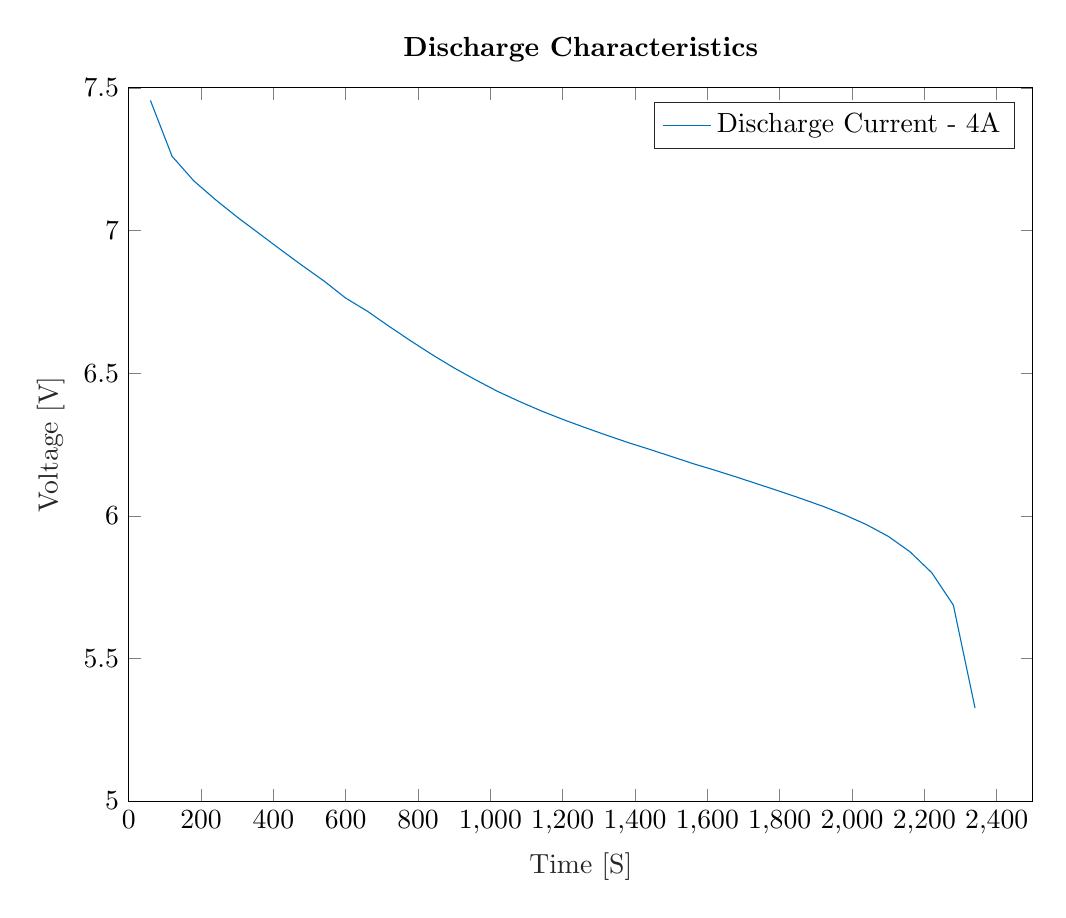
\begin{tikzpicture}

\begin{axis}[%
width=4.521in,
height=3.566in,
at={(0.758in,0.481in)},
scale only axis,
xmin=0,
xmax=2500,
xlabel style={font=\color{white!15!black}},
xlabel={Time [S]},
ymin=5,
ymax=7.5,
ylabel style={font=\color{white!15!black}},
ylabel={Voltage [V]},
axis background/.style={fill=white},
title style={font=\bfseries},
title={Discharge Characteristics},
legend style={legend cell align=left, align=left, draw=white!15!black}
]
\addplot [color=mycolor1]
  table[row sep=crcr]{%
60	7.456\\
120	7.26\\
180	7.174\\
240	7.108\\
300	7.047\\
360	6.99\\
420	6.933\\
480	6.877\\
540	6.823\\
600	6.763\\
660	6.717\\
720	6.664\\
780	6.613\\
840	6.564\\
900	6.518\\
960	6.476\\
1020	6.436\\
1080	6.401\\
1140	6.368\\
1200	6.338\\
1260	6.31\\
1320	6.283\\
1380	6.257\\
1440	6.233\\
1500	6.208\\
1560	6.183\\
1620	6.16\\
1680	6.136\\
1740	6.111\\
1800	6.086\\
1860	6.06\\
1920	6.033\\
1980	6.003\\
2040	5.969\\
2100	5.928\\
2160	5.874\\
2220	5.801\\
2280	5.687\\
2340	5.326\\
};
\addlegendentry{Discharge Current - 4A}

\end{axis}
\end{tikzpicture}%
	\caption{Discharge curve of the Ansmann 18650 2S1P Li-Ion battery used to power the swarmbot.}
	\label{fig:discharge_repeat}
\end{figure}
According to \cite{microzed_hardware_guide} the estimated maximum power draw of the MicroZed is 1.7A at 5V.
This is assuming 85\% utilisation of PL and a conservative 80\% efficiency of the converters.
The estimate made by Avnet is made with the Zynq-7010 in the Xilinx Power Estimator (XPE) \cite{xpe}.
The MicroZed used for the swarmbot project, however, is equipped with the Zynq-7020, a slightly larger chip.
Running the same scenario, 85\% utilisation, in XPE reveals that the 7020 draws 2.3W, just 0.1W more than the 7010, a marginal difference in the total power budget.
In addition to the MicroZed, also the debug LEDs and the microphone board are powered from this rail, adding an estimated $\approx$150mA extra current draw.
In summary, these are the requirements for the DC/DC converter used for generating the 5V rail:

\begin{itemize}
	\item Must function across the entire voltage range of the battery, 6V to 8.4V.
	\item Should be able to supply at least 1.85A at 5V.
\end{itemize}

Below is a discussion of the various choices made in the design of the circuitry of the 5V supply.

\subsubsection*{Designing the 5V Rail}
The PTH08080WAH \cite{pth08080} closely meets these requirements at a maximum power delivery of 2A/10W/5V.
The device is designed to have a wide input range, accepting \texttt{Vin}=\texttt{Vo}+1.1V to 18V.
At the required 5V this translates to an input range of 6.1V to 18V.
This is of course slightly higher than the desired 6V, but even at the maximum discharge rate, estimated at 2.2A-2.3A, with the MicroZed drawing its maximum current and the motors running at full speed, there would still be approximately 70 minutes of operation per charge.
\texttt{Vo} is determined via an external resistor \texttt{Rset}.
A formulae is provided to calculate the exact \texttt{Rset} needed for a given voltage, however a large table of common values is already calculated.
According to this table, \texttt{Rset}=353$\Omega$ results in 5V.
353$\Omega$ is not a standard value, choosing 348$\Omega$ instead yields 5.01V, which is fine for this application.
\\~\\
The circuit appertaining to this component can be seen in figure \ref{fig:pth08080}.
This is the standard application circuit as shown in the datasheet (figure 10 \cite{pth08080}).
According to the datasheet, the minimum recommended input capacitance is 100$\mu$F. 
Of the capacitors on the list of recommended capacitors, also given in the datasheet, the 20SVP150M was chosen.
It is rated for 20V, sufficient for this application, and has a capacitance of 150$\mu$F. 
\begin{figure}[h]
	\centering
	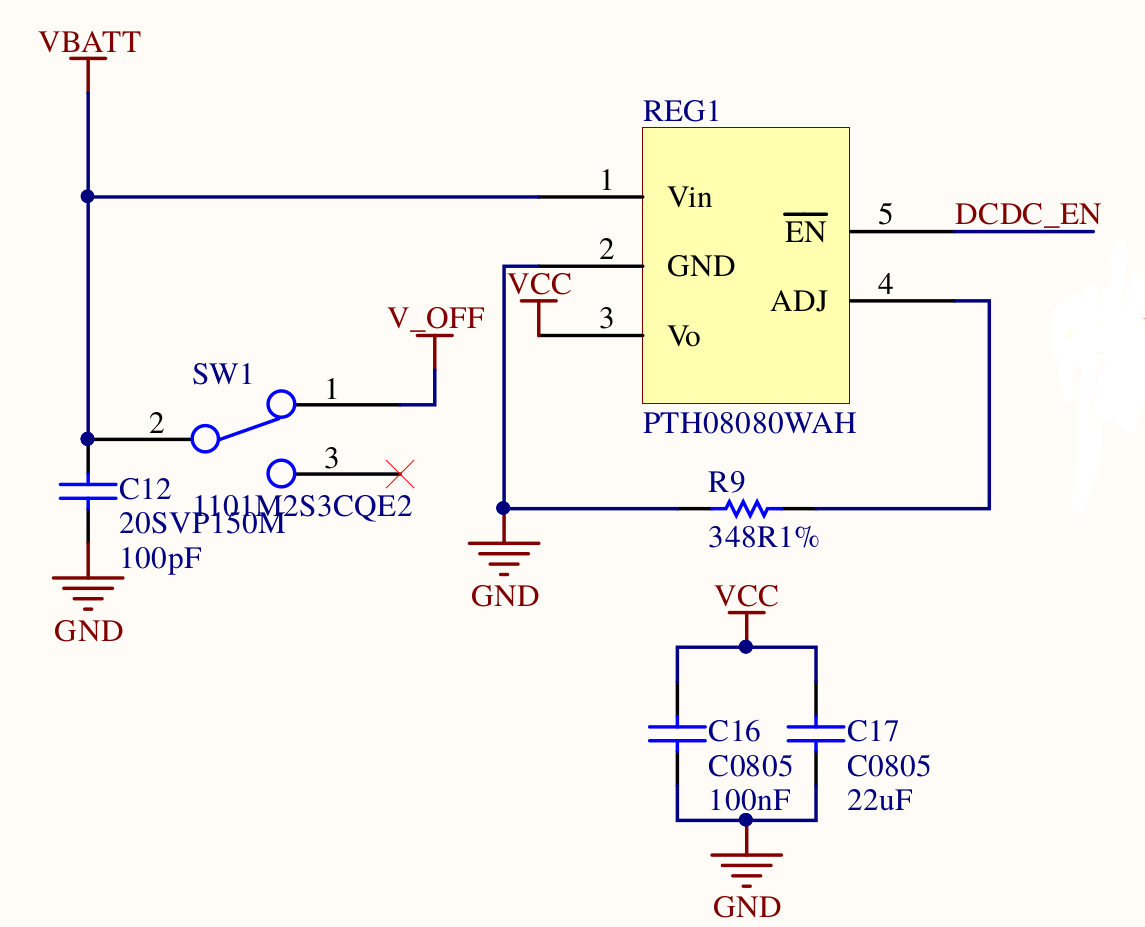
\includegraphics[width=0.6\linewidth]{graphics/5v.png}
	\caption{Circuit for generating \texttt{VCC}, the 5V rail.}
	\label{fig:pth08080}
\end{figure}
\mikkel{Prettify figure images (remove stupid things), make png and update enable pin to inhibit}

\subsection{Power Up Sequence} % (fold)
\label{sub:power_up_sequence}
According the carrier card design guide, \cite{design_carrier}, a carrier card needs to adhere to a specific power up sequence in order for the MicroZed to turn on correctly.
On power up, MicroZeds \texttt{PWR\_EN} signals need to be pulled high on the carrier card, to enable power to the MicroZed.
This is done with a pull-up resistor as shown in figure \ref{fig:pwr_en_circuit}.

\begin{figure}[h]
	\centering
	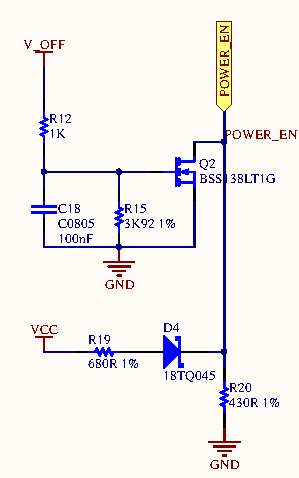
\includegraphics[width=.3\linewidth]{graphics/power_en_sch.pdf}
	\caption{Circuit for proper power sequencing on MicroZeds PWR\_EN.}
	\label{fig:pwr_en_circuit}
\end{figure}

When the MicroZed has powered up its internal DC/DC converters and is ready to receive voltage on its I/O banks \texttt{VCCIO\_EN} will go high.
\texttt{VCCIO\_EN} has a logic level of 1.8V and the signal is therefore fed to a comparator that outputs a 5V signal to a DC/DC converter when \texttt{VCCIO\_EN} is high.
The DC/DC converter is configured to produce a voltage level of 3.3V that is connected to \texttt{VCCIO}.
This circuitry can be seen in figure \ref{fig:pwr_io_circuit}.

\begin{figure}[h]
	\centering
	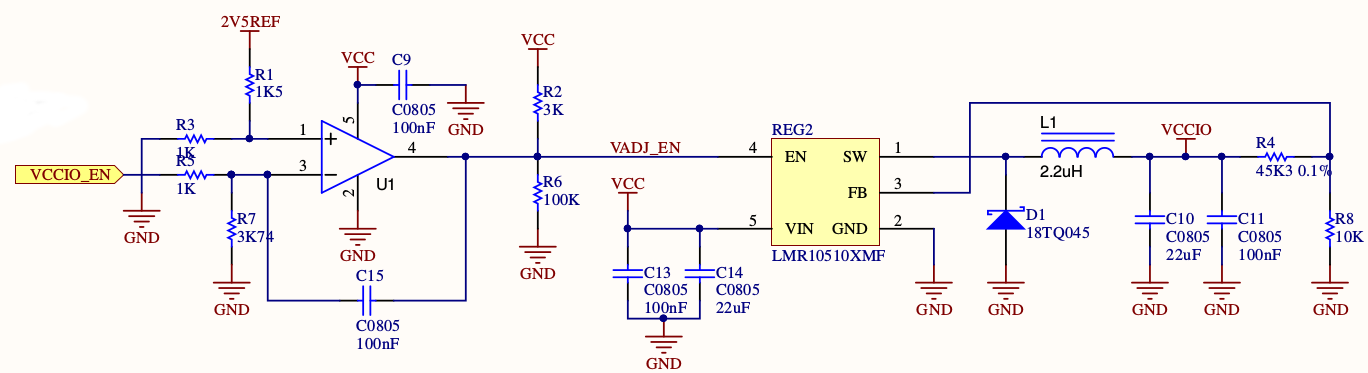
\includegraphics[width=1\linewidth]{graphics/vccio_power_up.png}
	\caption{Circuit for proper power sequencing on I/O banks.}
	\label{fig:pwr_io_circuit}
\end{figure}

% subsection power_up_sequence (end)
\subsection{Power Down Sequence} % (fold)
\label{sub:power_down_sequence}
A power down sequence is also described in \cite{design_carrier}, that needs to be followed to ensure signal integrity while powering down. 
The signals \texttt{VCCIO\_EN}, \texttt{DCDC\_EN} and \texttt{PWR\_EN} should be pulled down in that order when powering off.
The signals are pulled down by mosfets controlled by the \texttt{V\_OFF} signal.
When the power switch on the carrier card is in off mode, the battery voltage is connected to the \texttt{V\_OFF} rail thereby turning the mosfets on and pulling the signals down. 
The correct sequence is maintained by charging capacitors on the gate side of the mosfets thereby creating a delay.
Such a mosfet circuit is shown in figure \ref{fig:pwr_en_circuit}.
% subsection power_down_sequence (end)
\subsection{Analog to Digital Converter} % (fold)
\label{sub:analog_to_digital_converter}
The Zynq 7-series FPGA's are equipped with a dual, 12 bit ADC, yet has only one dedicated analog differential pair, \texttt{VP\_0} and \texttt{VN\_0}.
See figure \ref{fig:adc} for an overview of the XADC architechture
If more ADC channels are needed, any of the 16 auxiliary analog inputs (AAI) can be used.
These are placed on I/O bank 35 which, as the rest of the I/O on the swarmbot carrier card, is supplied with \texttt{VCCIO}=3.3V.
Once selected, a multiplexer applies each signal to the ADC's in turn.
For this reason any signal on the AAI can never go above \texttt{VCCIO} to avoid damaging the inputs.
On the swarmbot carrier card the dedicated analog pins, as well as three AAI pairs are routed to the ADC header (\texttt{CON4}).
The signals \texttt{VAUX\_P0} and \texttt{VAUX\_N0} on \texttt{JX1} are the dedicated analog inputs and can be used on its own.
The remaining three pairs are AAI and must be multiplexed if the user wishes to use them.
It should be noted that due to the anti-aliasing filters, these pairs cannot be used as digital I/O on the swarmbot carrier card.
These anti-aliasing filters are required in order to filter out high frequency noise in the differential pairs and should be placed as closely to the Zynq as possible, in this case, that is next to the connectors \texttt{JX1} and \texttt{JX2}, the main connectors to the MicroZed.
Figure \ref{fig:anti_a} from \cite{adch} illustrates a simple measurement setup and the anti-aliasing filter.
\texttt{R1} and \texttt{R2} form a voltage divider, creating a 1V signal.
\texttt{R5} is matched to the parallel impedance of \texttt{R1||R2}.
Resistors \texttt{R3}, \texttt{R4} and the capacitor \texttt{C1} can be adjusted to change the settling time of the circuit.
\cite{adc} gives equation \ref{eq:aliasing} which can be used to calculate the settling time and by that determine the maximum sampling frequency.

\begin{equation}
	\label{eq:aliasing}
	T_{s}=\ln{2^{resolution+1}}\cdot \left(\frac{R1\cdot R2}{R1 + R2}+R3+R4+R5\right)\cdot C_1 = 4.9\cdot 10^{-6}[\text{S}]
\end{equation}

\begin{figure}[h]
	\centering
	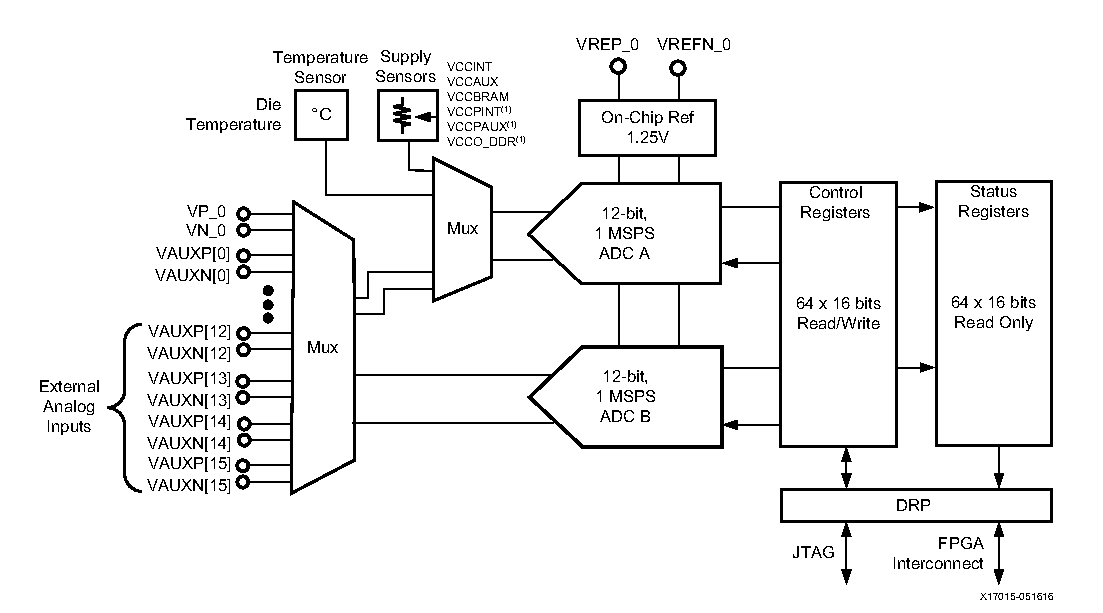
\includegraphics[width=1\linewidth]{graphics/adc.pdf}
	\caption{XADC Block Diagram from Xilinx ADC userguide \cite{adc}.}
	\label{fig:adc}
\end{figure}

\begin{figure}[h]
	\centering
	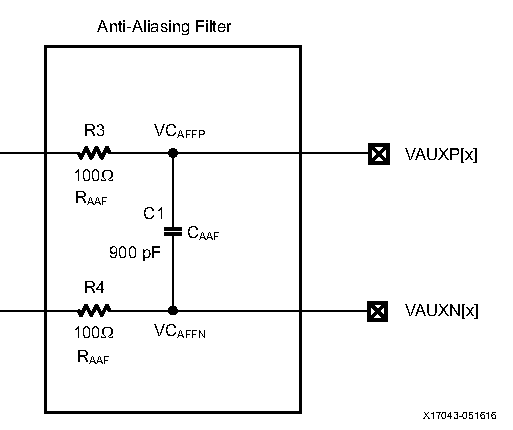
\includegraphics[width=0.8\linewidth]{graphics/anti_aliasing.pdf}
	\caption{Anti-Aliasing diagram from Xilinx ADC userguide \cite{adc}.}
	\label{fig:anti_a}
\end{figure}
% subsection analog_to_digital_converter (end)
\subsection{Buzzer Solution}	
As described in section \ref{sub:click_generator} it was found that the best solution for creating a clicking noise on the platform was to use a piezo speaker with a drive circuit and a \texttt{PWM} signal.
But because there has been made no further investigation into what sound level is needed and what the frequency spectrum of the generated click is, it was decided to leave the circuitry out of the carrier card.
Furthermore the sound source should be placed in the center of the robot to ease localization of the robot, but the design of the carrier card did not allow this.
Therefore it was decided to include a header providing access to two IO ports, ground and \texttt{VBATT}.
The header is shown in figure \ref{fig:audio_header}.
Two IO ports are needed if differential drive of the piezo is wanted.
Two holes were added to the carrier card to allow for fixture of the external piezo and drive circuit.

\begin{figure}[h]
	\centering
	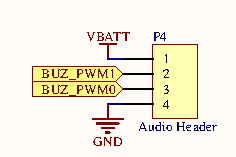
\includegraphics[width=0.4\linewidth]{graphics/audio_header.pdf}
	\caption{Audio header on the carrier card.}
	\label{fig:audio_header}
\end{figure}

\subsection{Pinout}


\subsection{Choice of Components}
As mentioned, the choice of components is largely based upon the Avnet carrier card.
Generally the same components were chosen but due pricing, availability or minimum order size, some components were changed to similar ones.
Table \ref{tab:components1} and \ref{tab:components2} in appendix \ref{app:components} explains what components were chosen and why.

\subsection{Swarmbot Carrier Card Layout} % (fold)
\label{sub:swarmbot_carrier_card_layout}
The layout of the swarmbot carrier card was done using Altium Designer.
From an early stage it was decided to have the board manufactured by a professional outlet as this would both greatly ease the layout process and, hopefully, minimize the potential points of failure in debugging process.
The former, a simpler layout process, is expected for a number of reasons outlined below:
\begin{itemize}
  	\item \textbf{Mutlilayer Board:} Due to the size constraints of the board it is desirable to minimize the number of traces that are required to be routed on the board.
  	Creating a 4-layer board means that the two middle layers can be \texttt{GND} and \texttt{VCC}, allowing every connection to either of these plains to be done using a simple via.
  	\item \textbf{Feature Size:} The manufacturing method used at SDU is not reliable at tracewidths below 20mil and all vias must be drilled by hand, resulting in signal traces being far wider than what is actually required.
  	The manufacturer used to produce the swarmbot carrier card \cite{itead} allows traces as low as 8mil and vias at 12mil.
  	\item \textbf{Plated Vias:} The vias created by the manufacturer are plated with copper, meaning that, when using throughhole components the trace can be routed on both the top and bottom layers, without the use of additional vias.
  	This greatly reduces the number of vias required for the layout.
  \end{itemize}
Finally, as was alluded to in the previous paragraphs, the manufacturing process at SDU is not particularly robust and often requires several attempts before the correct combination of incantations, candles and luck is found and a fully functional board is created.
\\~\\
The board has three trace widths: 40mil for \texttt{VBATT}, 20mil for \texttt{VCCIO} and 8mil for the remaining signal wires.
Mostly, the size of the board is due to the number of connectors that are required.
For this reason there is plenty of room for components and generally capacitors and resistors were chosen with a 0805 footprint.
The anti-aliasing filters described in section \ref{sub:analog_to_digital_converter} are required to be placed close to the Bergstak connectors (the connector for mounting the MicroZed), which has a 0.8mm pitch.
Using 0805 components here is infeasible due to size and it was decided to use 0402 instead.
% subsection swarmbot_carrier_card_layout (end)